\documentclass[10pt]{article}
\usepackage[margin=0.85in,headheight=13pt]{geometry}
\usepackage[utf8]{inputenc}
\usepackage{microtype}
\usepackage{amsmath,amssymb}
\usepackage{graphicx}
\usepackage{booktabs}
\usepackage{array}
\usepackage[numbers,square,sort&compress]{natbib}
\usepackage{hyperref}
\usepackage{placeins}
\usepackage{fancyhdr}
\usepackage{xcolor}
\hypersetup{colorlinks=true,linkcolor=blue!45!black,citecolor=blue!45!black,urlcolor=blue!45!black}
\setlength{\parindent}{0pt}
\setlength{\parskip}{0.45em}
\setlength{\emergencystretch}{2em}
\pagestyle{fancy}
\fancyhf{}
\fancyhead[L]{Data Shapley for training-data valuation}
\fancyhead[R]{Assignment 9}
\fancyfoot[C]{\thepage}
\renewcommand{\headrulewidth}{0.3pt}
\newcommand{\low}{\textsc{Low}}
\newcommand{\rand}{\textsc{Random}}
\newcommand{\high}{\textsc{High}}

\title{\vspace{-2.5em}
\includegraphics[width=2.6cm]{unimi_logo.png}\\[0.8em]\textbf{Which training points help, and which hurt?}\\
\large Data Shapley on clean and noisy data}
\author{Diana Amirian\\
Statistical Methods for Machine Learning, Assignment 9\\
Universit\`a degli Studi di Milano}
\date{October 2026}

\begin{document}
\maketitle
\vspace{-1em}

\section*{Summary}
I estimated a Data Shapley value for every training point with permutation sampling, using a 3-nearest-neighbour classifier written from scratch, and then removed the lowest-value points, the highest-value points or random points. The experiment was repeated on ten seeds for three conditions: clean Penguins, Penguins with 20\% of training labels flipped, and a two-class Gaussian dataset with 20\% of training labels flipped.

With label noise, removing the lowest-value 20\% of the training set raised mean test accuracy by 8.51 percentage points over random removal on Penguins and by 8.88 points on the Gaussian data, and \low{} beat \rand{} in all ten runs of both. On clean Penguins it showed no clear average advantage: $-0.04$ points, with an interval that includes zero. Removing the highest-value points lowered mean accuracy in every condition. Low values also pointed to the flipped labels: the mean AUROC for finding them was 0.993 on Penguins and 0.851 on the Gaussian data. The weak spots are the clean-Penguins ranking, which stays unstable, and one run where removing 40\% left almost no Chinstrap training points.

\section{What is Data Shapley?}
A model is usually judged as a whole, by its accuracy or loss. Data Shapley \citep{ghorbani2019} asks a different question: how much does each single training point contribute to that performance? It borrows the answer from cooperative game theory. The training points are the players, and the ``payoff'' of a team $S$ of points is the performance $V(S)$ of a model trained on $S$. The Shapley value \citep{shapley1953} of point $i$ is its average marginal contribution:
\[
\phi_i=\frac{1}{n}\sum_{S\subseteq N\setminus\{i\}}\binom{n-1}{|S|}^{-1}\Big[V\big(S\cup\{i\}\big)-V(S)\Big],
\]
where $N$ is the training set of size $n$. Equivalently, $\phi_i$ is the average gain from adding $i$, taken over all $n!$ orders in which the points could arrive. A point may help when added to one subset and hurt when added to another; its value averages these effects. Positive and negative values therefore describe average contributions to the chosen utility. A negative value does not guarantee that removing the point from the full training set improves performance.

The Shapley value satisfies four properties: points with identical contributions receive equal values (symmetry), a point that never changes the score receives zero (null player), values add when utilities are added (additivity), and all values sum to $V(N)-V(\emptyset)$ (efficiency). Exact enumeration would require evaluating $2^n$ subsets, which is infeasible here for $n=205$, so I estimate the values by sampling random orders.

The paper reports that low-value points are often harmful, for example mislabelled, and that removing them can improve a model. This project estimates the values by permutation sampling for a k-NN classifier, as the assignment asks, and checks two of these claims on a small real dataset and a synthetic dataset with label noise: whether removing low-value points gives better test accuracy than removing the same number of random points, and whether flipped labels end up with low values. Section~\ref{sec:paper} compares the findings with the paper.

\section{Data}
\textbf{Penguins.} The real dataset is Palmer Penguins \citep{horst2020,gorman2014}. It has 344 rows. Two rows miss all four measurements and are dropped, leaving 342 penguins: 151 Adelie, 123 Gentoo and 68 Chinstrap. The features are bill length, bill depth, flipper length and body mass, and the target is species. I chose it because it is small, clean, multiclass and freely licensed, so every step can be checked by hand and the Shapley computation stays fast. For each seed the data is split by species (stratified, so every class keeps approximately the same share in each part) into 205 training, 68 validation and 69 test points (about 60/20/20). The noisy version uses the same split and changes exactly 41 training labels (20\%) to one of the other two species, chosen uniformly. This is the uniform (symmetric) label-noise model, and 20\% is the flip rate the paper uses in its spam experiment. Validation and test labels are never changed.

\textbf{Gaussian data.} The synthetic dataset has two balanced classes,
\[
X\mid Y=0\sim\mathcal{N}\big((-1,0),I_2\big),\qquad X\mid Y=1\sim\mathcal{N}\big((1,0),I_2\big).
\]
The classes overlap, so even the best possible classifier makes mistakes: with equal priors the Bayes rule predicts by the sign of the first coordinate, and its error is $\Phi(-1)\approx 15.9\%$. Each seed draws 150 training, 90 validation and 1,000 test points. The test set is large because it costs nothing during valuation. Exactly 30 training labels (20\%) are flipped. Since I generate the data, I know exactly which labels are wrong, which makes it a clean test of whether Shapley values find them.

\textbf{Scaling.} Features are standardized with the training mean and standard deviation only, and the same numbers are used for validation, test and every removal. Scaling matters for k-NN because distances are dominated by the feature with the largest units, here grams over millimetres. Fitting the scaling on the training part only keeps the validation and test sets unseen.

\begin{table}[!ht]
\centering\small
\caption{Data in each run.}
\label{tab:partitions}
\begin{tabular}{@{}lrrrr@{}}
\toprule
Condition & Train & Validation & Test & Flipped labels \\
\midrule
Clean Penguins & 205 & 68 & 69 & 0 \\
Noisy Penguins & 205 & 68 & 69 & 41 \\
Noisy Gaussian & 150 & 90 & 1,000 & 30 \\
\bottomrule
\end{tabular}
\end{table}

\section{Method}
\subsection{Classifier and utility}
The classifier is a 3-nearest-neighbour classifier written with NumPy only. k-NN is allowed by the assignment and avoids iterative parameter fitting, although every subset still requires neighbour selection, voting and validation scoring. Using $k=3$ gives a small local majority vote; it is fixed throughout the study, and no comparison of different $k$ values is made. Distances are Euclidean on the scaled features. Points tied at the third-nearest distance share the votes left after closer points have voted, so predictions do not depend on row order. This preserves the symmetry of identical training points in the underlying game. A class-vote tie goes to the class with the closest point; any remaining tie uses sorted class order. With fewer than three training points, all of them vote. Scaling is fitted once on the full training set and kept fixed for every subset, so the values refer to this fixed feature representation.

The utility $V(S)$ is the validation accuracy of 3-NN using the training points in $S$. An empty set cannot supply neighbours, so I define $V(\emptyset)$ as the validation accuracy of always predicting the majority class of the original clean training labels. These labels are available because the noise is injected artificially. This keeps the empty-set reference the same for clean and noisy Penguins within each seed. It is a simulation choice; an application without known clean labels would need a reference based on available information. Nonempty subsets use the observed training labels. The test set is reserved for evaluating removal, following the paper's separation between the set used for valuation and the held-out set used for final evaluation.

\subsection{Monte Carlo Data Shapley}
For a random order $\pi$ of the training points, let $S_i^\pi$ be the points before $i$. The contribution of $i$ in that order is $V(S_i^\pi\cup\{i\})-V(S_i^\pi)$, and the estimate after $t$ orders is
\[
\widehat{\phi}_i^{\,t}=\frac{1}{t}\sum_{m=1}^{t}\Big[V\big(S_i^{\pi_m}\cup\{i\}\big)-V\big(S_i^{\pi_m}\big)\Big].
\]
This permutation-sampling estimator is also used in the Data Shapley paper. For a fixed number of uniformly drawn orders the average is unbiased, and its error bound shrinks as more orders are drawn \citep{maleki2013}. Here the number of orders depends on the estimates through the stopping rule below, so the fixed-budget unbiasedness and error guarantees are not established for this adaptively stopped estimate. The error also need not fall at every checkpoint. Every order is evaluated to the end, without the truncation of the paper's TMC-Shapley, as the assignment asks for permutation sampling. The contributions in one order always add up to $V(\text{all})-V(\emptyset)$ (the efficiency property), which the code checks.

To decide when to stop, I use an adapted version of the convergence rule from the paper \citep{ghorbani2019}. Let $I_t=\{i:\widehat{\phi}_i^{\,t}\ne 0\}$ be the points with a nonzero current estimate. For $I_t\ne\emptyset$, the stopping condition is
\[
\frac{1}{|I_t|}\sum_{i\in I_t}\frac{\big|\widehat{\phi}_i^{\,t}-\widehat{\phi}_i^{\,t-100}\big|}{\big|\widehat{\phi}_i^{\,t}\big|}<0.05 .
\]
Points whose estimate is exactly zero are excluded because the ratio is undefined for them; if all current estimates are zero, the code assigns the statistic a value of zero. This rule measures recent changes in the estimates and does not give a formal bound on their error. The rule is checked every 100 orders, but only after a minimum number of orders. This makes it less likely to pass by chance early on, although it cannot rule that out. There is also a cap of 20,000 orders, which no run reached.

The minimum comes from a pilot on seed 100 that does not score the test set. Two independent sampling streams per condition were compared at 50, 100, 200 and 500 orders, using Spearman rank correlation of at least 0.90 and bottom-set overlap of at least 0.80 as descriptive references. Clean Penguins missed these, so the pilot continued to 1,000 and 2,000 orders. Its rankings still disagreed at 2,000. I therefore use 2,000 as a practical minimum budget, not as evidence of stable rankings, and then apply the adaptive stopping rule. Appendix A.1 checks ranking stability separately.

Evaluating every prefix of every order is slow if distances are recomputed each time. For k-NN, the prediction for a query depends only on the order of the training points by distance to it, which is also the idea behind the exact k-NN Shapley algorithm of \citet{jia2019knn}. That algorithm runs in $O(N\log N)$ per validation point, but for a different utility: the share of the $K$ nearest neighbours that have the correct label. I use the accuracy of the final majority vote as the utility, so their formula does not apply directly. The fast evaluator therefore computes and sorts the distances from each validation point once, then only marks which training points are present as an order grows. It gives exactly the same prefix accuracies as the simple version: all 56,300 were compared (Appendix A.2). On this machine it was 18 to 19 times faster.

\subsection{Removal and uncertainty}
In each run the points are ranked once by their estimated value. Exact ties between stored floating-point estimates are broken by a seeded random order. At 10, 20, 30 and 40\% removal, \low{} removes the lowest values and \high{} removes the highest, as in Fig.~1 of the Data Shapley paper, and \rand{} removes the same number of points chosen at random, repeated 30 times and averaged within the run. 3-NN is then retrained on what is left and scored on the test set. The ranking and the scaling are not recomputed after removal.

The main comparison is \low{} minus \rand{} within each run, averaged over ten runs. Pairing compares strategies on the same split and noise realization; the 30 random-removal scores are averaged before taking the difference. The 95\% intervals use 5,000 bootstrap resamples of the ten run-level differences \citep{efron1993}. They describe the estimated variability of the mean difference, while standard deviations describe variation between runs. The intervals are descriptive: the Penguins runs are repeated splits of the same 342 observations, not ten independently collected datasets. Such reuse limits population-level interpretation and can make intervals too narrow \citep{nadeau2003}.

\subsection{Pipeline}
Figure~\ref{fig:flow} shows the order of the steps. The pilot first fixes the minimum number of permutations, using seed 100 and no test data. Then, for each seed, the data is split and scaled using training statistics, and the three conditions are built. Clean Penguins keeps its original labels; 20\% of training labels are flipped only in noisy Penguins and noisy Gaussian data. Shapley values are estimated from the training and validation sets, and the points are ranked. In the noisy conditions, label-noise detection compares these rankings with the known training-label corruption flags; it does not use the test set. Once the values and rankings for all three conditions are fixed, \low{}, \high{} and \rand{} subsets are removed and 3-NN is scored on the held-out test set. Finally the ten seeds are combined into the tables and figures, and a separate check regenerates the sampled orders and stopping points and recomputes every removal outcome.

\begin{figure}[!ht]
\centering
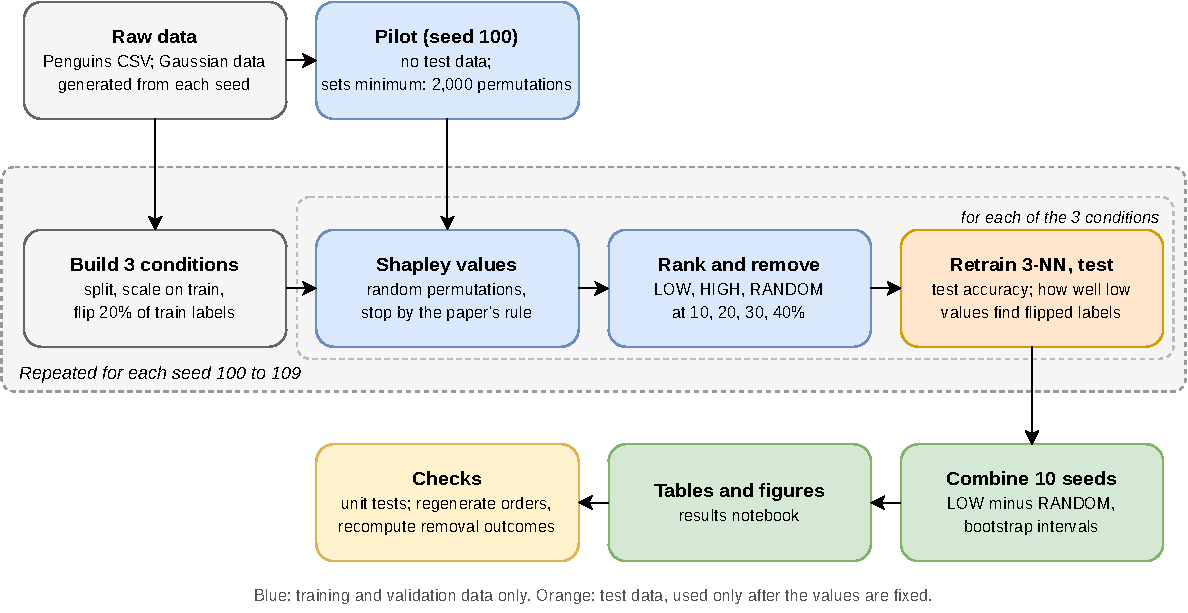
\includegraphics[width=0.9\linewidth]{flowchart.pdf}
\caption{The pipeline. Blue steps use training and validation data; label-noise detection also uses the known training-label corruption flags. Only the orange step uses the held-out test set, after values and rankings are fixed. Label flips are injected only in the two noisy conditions.}
\label{fig:flow}
\end{figure}

\section{Results}
\subsection{Number of permutations}
Every run met the convergence rule. Clean Penguins needed 2,800 to 3,400 orders. Noisy Penguins stopped at 2,000 in nine runs and 2,200 in one. Noisy Gaussian stopped at 2,000 in all runs. That clean Penguins needs the most matches the pilot: its values are small and close together, so they settle slowly.

\subsection{Accuracy after removal}
Figure~\ref{fig:removal} plays the role of Fig.~1 in the Data Shapley paper. On clean Penguins all three strategies stay close to the 98.84\% full-data accuracy. With label noise the three curves separate clearly: \low{} rises, \rand{} stays flat and \high{} falls.

\begin{figure}[!ht]
\centering
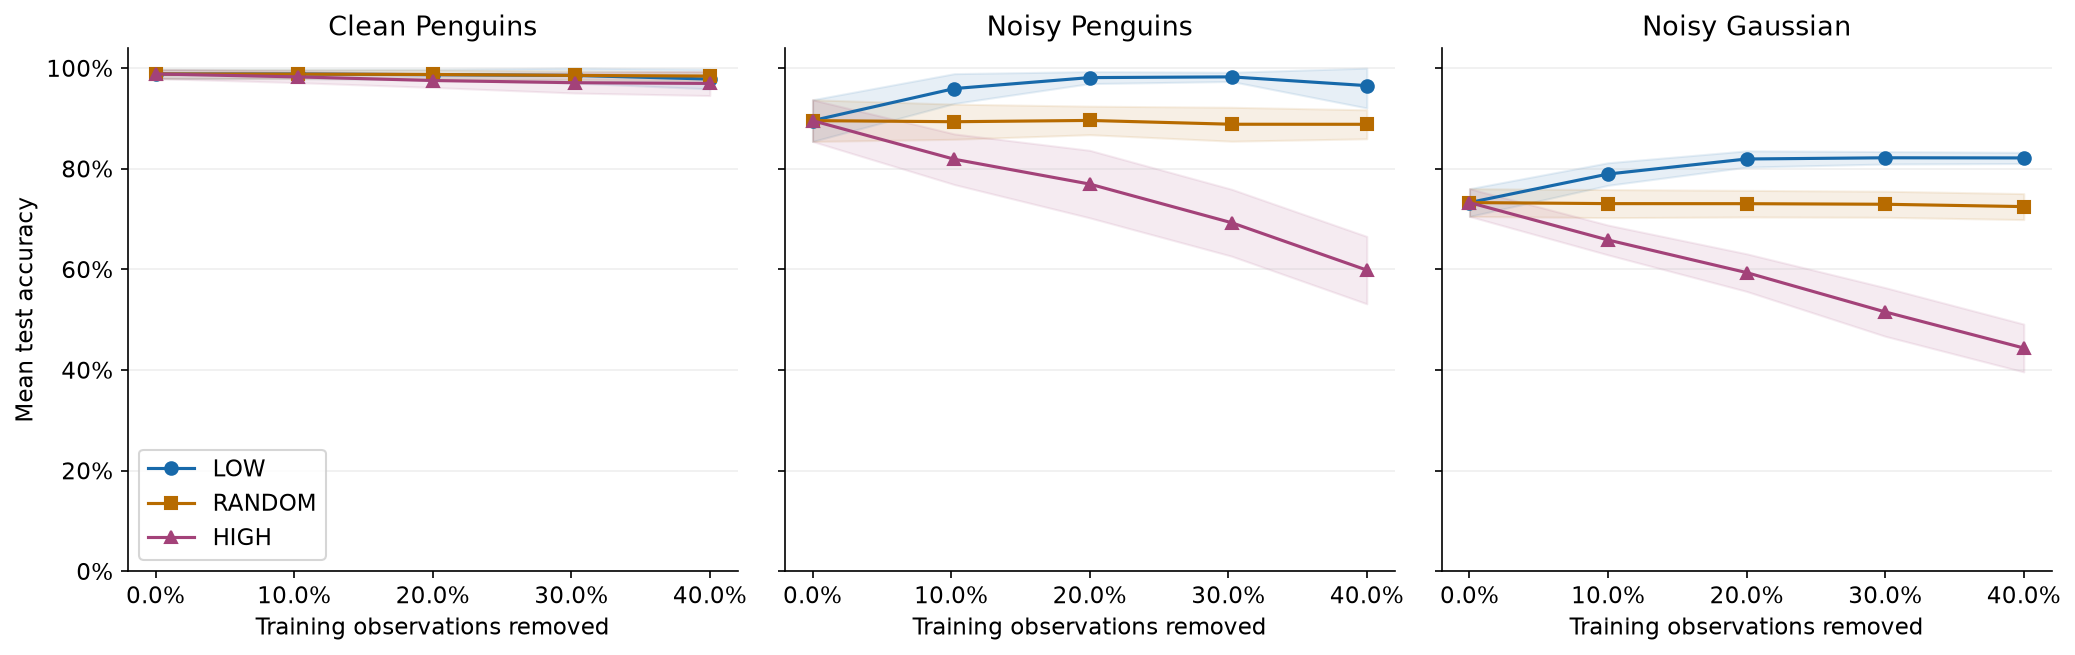
\includegraphics[width=\linewidth]{figures/study_accuracy.png}
\caption{Mean test accuracy over ten runs against the share of training points removed. Bands are $\pm$ one standard deviation across runs. For \rand{}, each run contributes the mean of its 30 random subsets.}
\label{fig:removal}
\end{figure}

\begin{table}[!ht]
\centering\small
\caption{Mean test accuracy at 20\% removal and the paired \low{} minus \rand{} difference in percentage points (pp). W/T/L counts the runs where \low{} wins, ties or loses against \rand{}.}
\label{tab:primary}
\begin{tabular}{@{}lrrrrrlc@{}}
\toprule
Condition & No removal & \low{} & \rand{} & \high{} & Difference & 95\% interval & W/T/L \\
\midrule
Clean Penguins & 98.84\% & 98.70\% & 98.74\% & 97.54\% & $-0.04$ & $[-0.39, +0.27]$ & 6/0/4 \\
Noisy Penguins & 89.57\% & 98.12\% & 89.60\% & 76.96\% & $+8.51$ & $[+7.05, +9.96]$ & 10/0/0 \\
Noisy Gaussian & 73.28\% & 81.94\% & 73.06\% & 59.36\% & $+8.88$ & $[+7.87, +9.96]$ & 10/0/0 \\
\bottomrule
\end{tabular}
\end{table}

Figure~\ref{fig:paired} shows the difference at every fraction. On noisy Gaussian data the gain grows from $+5.88$ points at 10\% to $+9.67$ at 40\%, and \low{} wins all 40 run comparisons. On noisy Penguins it is $+6.59$, $+8.51$, $+9.42$ and $+7.69$ points; \low{} wins every comparison except one run at 40\%, discussed in Section~\ref{sec:fail}. On clean Penguins the difference is $+0.03$, $-0.04$, $0.00$ and $-0.59$ points, and every interval includes zero.

\begin{figure}[!ht]
\centering
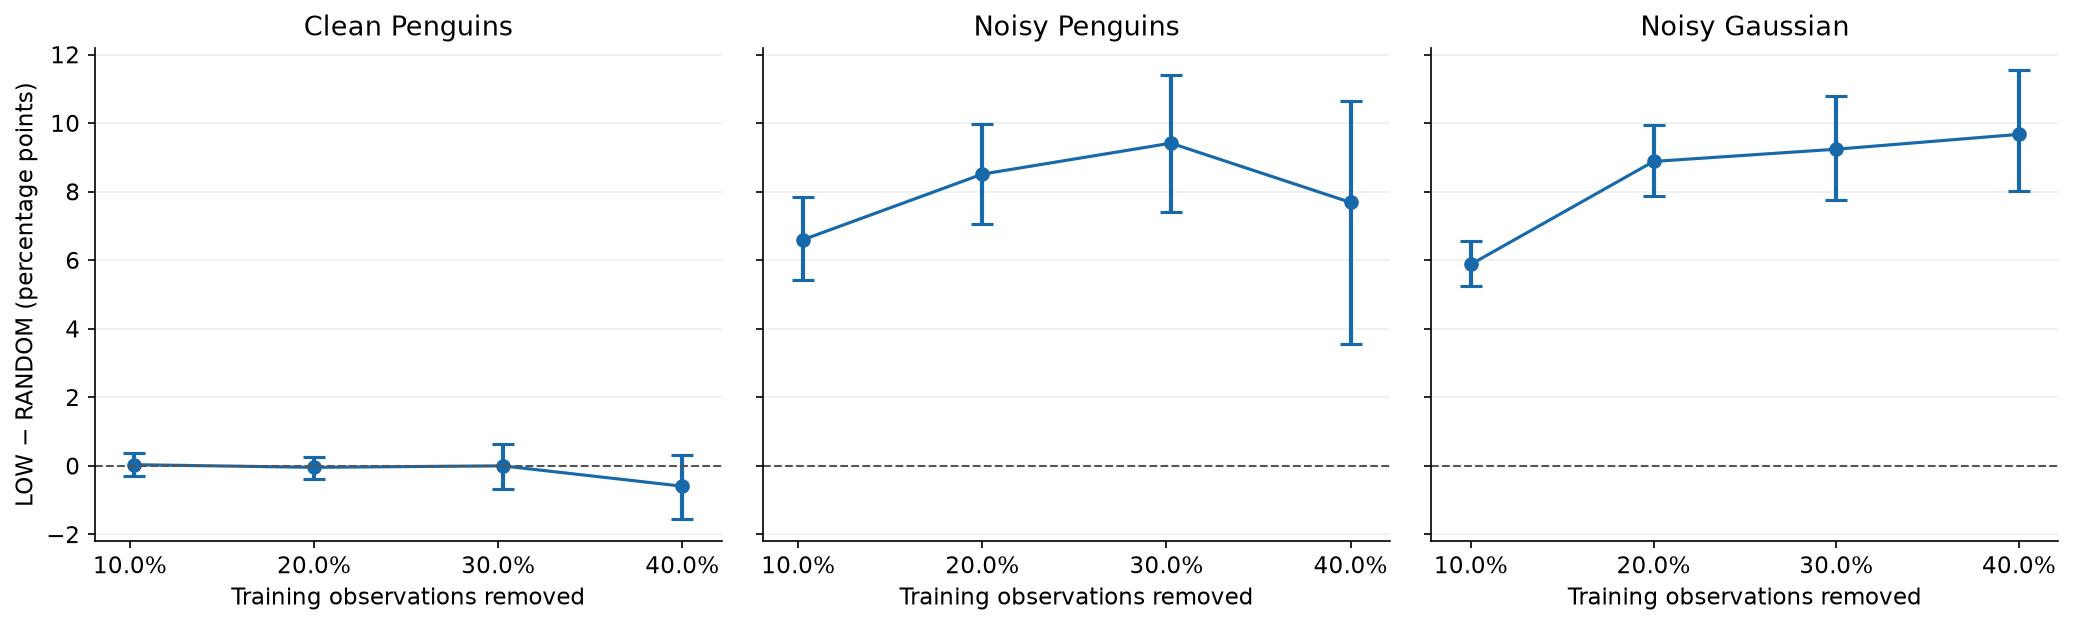
\includegraphics[width=\linewidth]{figures/study_paired_differences.png}
\caption{Mean \low{} minus \rand{} test accuracy over ten runs, with 95\% bootstrap intervals over runs. The dashed line is no difference.}
\label{fig:paired}
\end{figure}

\subsection{Distribution of values and flipped labels}
Figure~\ref{fig:values} shows the values. On clean Penguins they are small and almost all positive: only 2.2\% of all estimates are negative, between 0 and 9 points per run. With noise the flipped points move to the left. On noisy Penguins 96\% of flipped points have a negative value, against 2.8\% of the others. On noisy Gaussian data the figures are 80\% and 18\%. The larger overlap on the Gaussian data is consistent with its overlapping classes: correctly labelled points near the boundary can also have negative estimated contributions.

\begin{figure}[!ht]
\centering
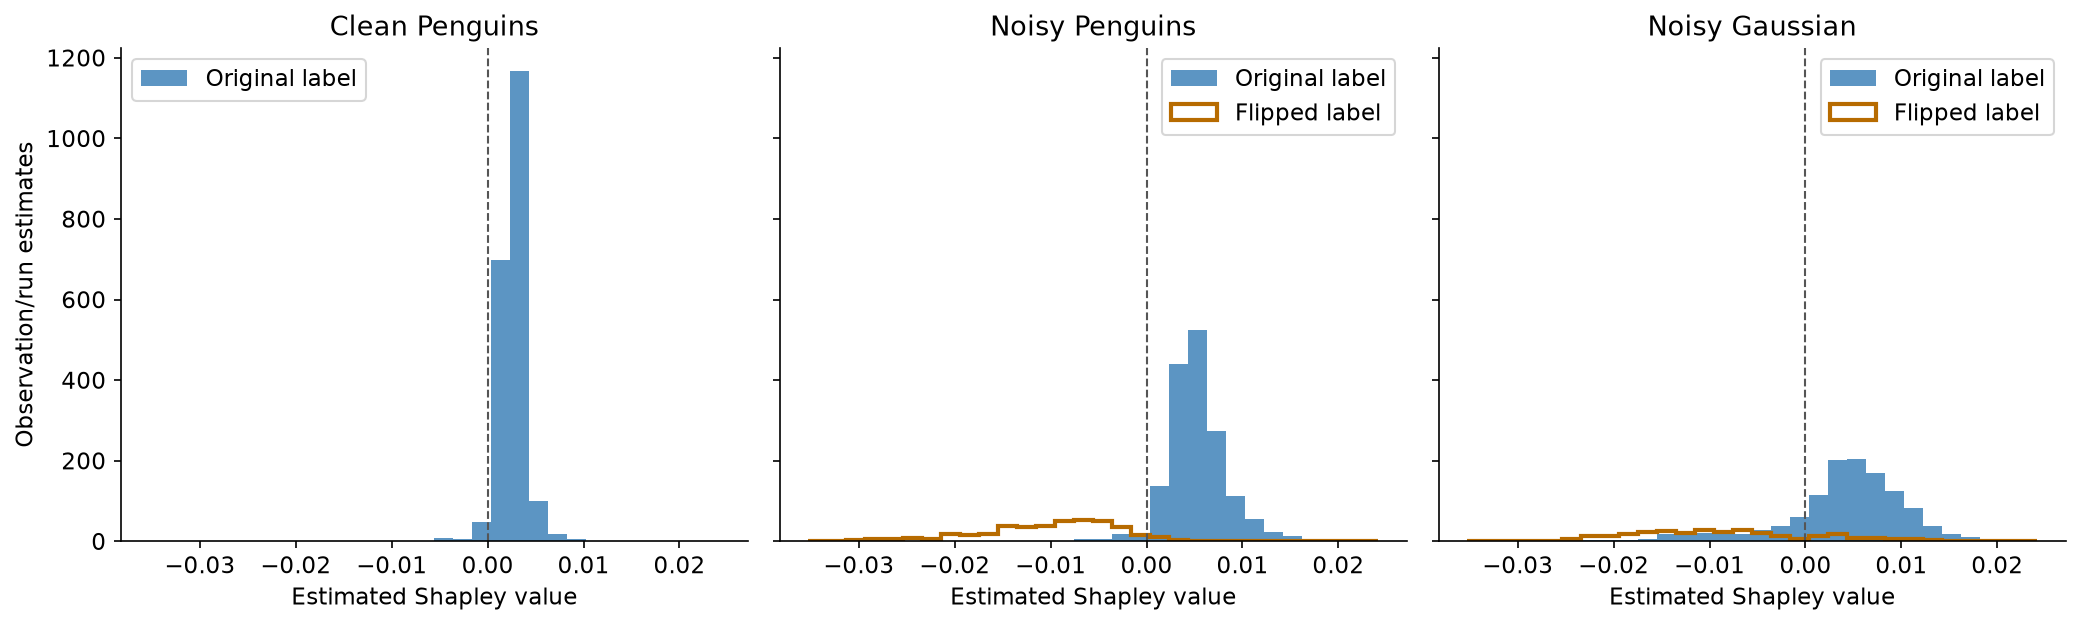
\includegraphics[width=\linewidth]{figures/study_value_distributions.png}
\caption{Shapley values pooled over the ten runs. Outlined bars are the flipped training points. Clean Penguins has none.}
\label{fig:values}
\end{figure}

If one checks points from the lowest value upward, as in the paper's label-noise experiment (Figure~\ref{fig:detection}), the mean AUROC for finding flipped labels is 0.993 (SD 0.006) on noisy Penguins and 0.851 (SD 0.058) on noisy Gaussian data; random checking would give 0.5. The AUROC is the probability that a random flipped point gets a lower value than a random correct one, with ties counted as half. Among the lowest 10\% of points, 100\% and 71\% are flipped. Among the lowest 20\%, which is the same number as the flips, the shares are 92.4\% and 63.3\%; random checking would give 20\%.

\begin{figure}[!ht]
\centering
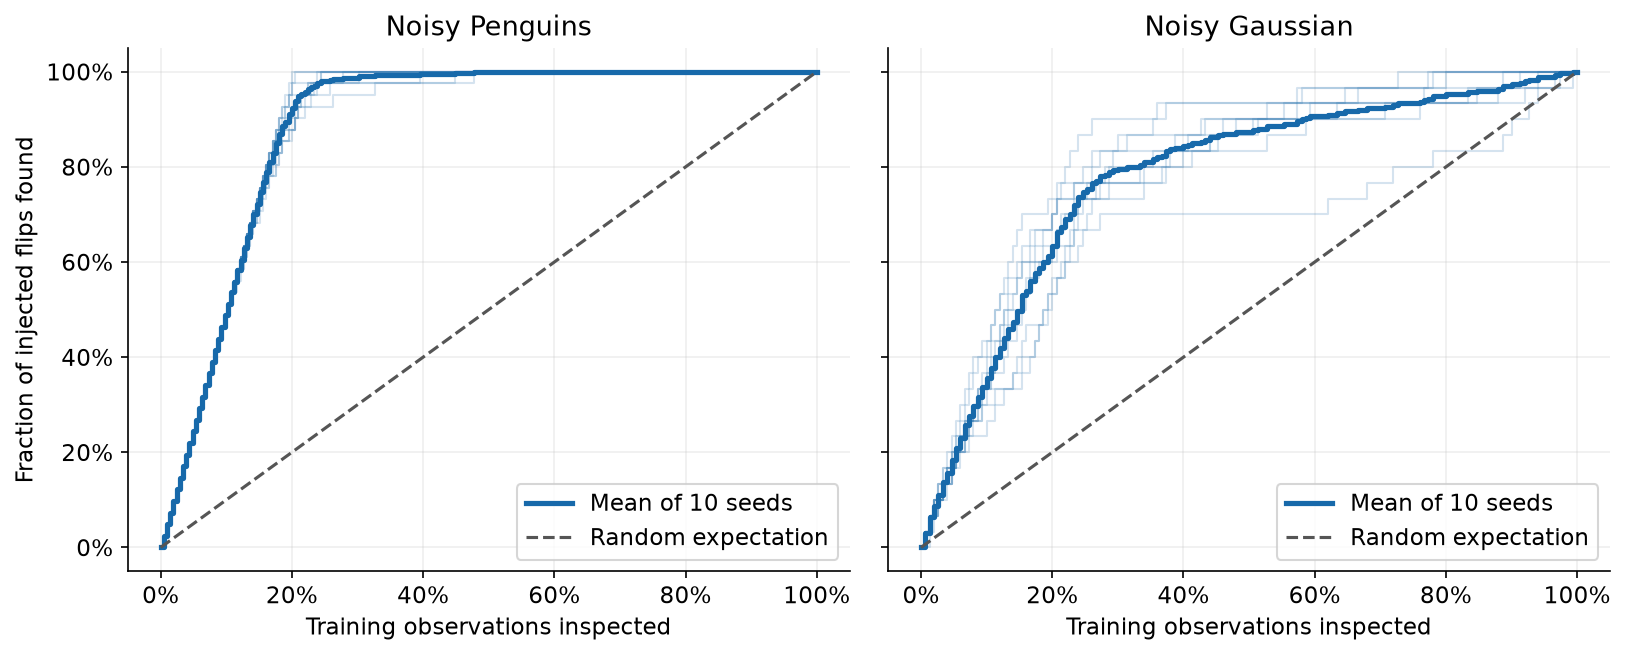
\includegraphics[width=\linewidth]{figures/study_detection.png}
\caption{Share of flipped labels found when checking training points from the lowest value upward. Thin lines are single runs, the thick line is their mean, and the diagonal is random checking.}
\label{fig:detection}
\end{figure}

\subsection{Comparison across the datasets}
The two noisy datasets give the same picture: a clear and consistent gain from removing low-value points, and a large loss from removing high-value ones. The Penguins gain at 20\% ($+8.51$) and the Gaussian gain ($+8.88$) are almost equal, but they mean different things. On noisy Penguins, \low{} brings accuracy back to 98.12\%, close to the clean 98.84\%, consistent with the high accuracy of flipped-label detection. On the Gaussian data, \low{} reaches about 82\%, below the population Bayes accuracy of about 84\% for this generating distribution. Here the flipped labels are harder to tell apart from honest points near the class boundary, which also explains the lower AUROC.

Clean Penguins is the opposite case. Accuracy starts at 98.84\%, and with 69 test points a single prediction is worth 1.45 points, so there is almost nothing to gain. At 20\% removal, \low{} left accuracy unchanged in nine runs and lost one test prediction in the tenth. Only a handful of points per run have a negative value, so removing 41 points also removes many points with small positive values. In this dataset ``low'' means ``least useful'', not ``harmful''.

\subsection{Ranking stability and a failure case}
\label{sec:fail}
The values for clean Penguins are noisy. In the pilot at 2,000 orders, the two independent streams had a Spearman correlation of 0.418 and shared 20 of their 41 bottom-20\% points; for noisy Penguins the figures were 0.938 and 40 of 41, and for noisy Gaussian 0.993 and 30 of 30. Even after the convergence rule passes, two independent clean-Penguins runs still disagree on many points (Appendix A.1). The 68-point validation set also limits how finely accuracy can separate points.

One noisy-Penguins run is an exception. For seed 104 at 40\% removal, \low{} reached 84.06\% against 91.74\% for \rand{}, because it also removed most of the smallest class, Chinstrap, and left only three Chinstrap-labelled training points (Appendix A.3). Removing a large share by value can empty a class, so class counts should be checked before removing aggressively.

\FloatBarrier
\section{Do the results match the paper?}
\label{sec:paper}
Table~\ref{tab:paper} puts the paper's main claims next to my results.

\begin{table}[!ht]
\centering\small
\caption{The paper's findings \citep{ghorbani2019} and my results (20\% removal, means over ten runs).}
\label{tab:paper}
\begin{tabular}{@{}>{\raggedright}p{0.30\linewidth}>{\raggedright}p{0.48\linewidth}l@{}}
\toprule
Paper & This project & Match \tabularnewline
\midrule
Removing high-value points hurts the model most (Fig.~1a) & \high{} lowers accuracy in every condition: 98.84\,$\to$\,97.54\% (clean), 89.57\,$\to$\,76.96\% (noisy Penguins), 73.28\,$\to$\,59.36\% (Gaussian) & Yes \tabularnewline
\addlinespace
Removing low-value points improves the model (Fig.~1b) & With label noise, \low{} beats \rand{} by 8.51 and 8.88 points, in all ten runs at 20\%. On clean Penguins: $-0.04$ points & Partly \tabularnewline
\addlinespace
Mislabelled points get low values and are found faster than by random checking (Fig.~3) & AUROC 0.993 and 0.851; the lowest 20\% hold 92.4\% and 63.3\% of the flips, against 20\% at random & Yes \tabularnewline
\addlinespace
Values converge within a few thousand permutations (2,000 to 5,000 in its experiments) & 2,000 to 3,400 per run, but the clean-Penguins ranking is still unstable & Mostly \tabularnewline
\bottomrule
\end{tabular}
\end{table}

The clearest difference in the removal results is clean Penguins, where removing low-value points showed no clear average benefit. The likely reason is the starting accuracy. In the paper's disease-prediction task, logistic regression on 1,000 patients and 285 features reached only 68.7\% and 56.4\%, so there was room to improve. Clean Penguins starts at 98.84\%, where one test prediction is worth 1.45 points and only 0 to 9 points per run have a negative value. With few negative estimates and an already high baseline accuracy, removing a fixed fraction also discards many points with positive estimated contributions. The setups also differ: the paper uses truncated Monte Carlo and models such as logistic regression and neural networks, while this project uses full permutations, an adapted version of its convergence rule, and 3-NN.

\section{Discussion}
\textbf{What worked.} The method did what the paper reports. Low values marked harmful points, here the flipped labels, and removing them improved accuracy on held-out data. High values marked the useful points, and removing them hurt much more than random removal. At 20\% removal these results held in all ten runs of both noisy datasets. The implementation was checked against exact Shapley values on small games, the fast evaluator matched the simple one exactly, and the saved orders, stopping points and removal outcomes can all be regenerated from the seeds.

\textbf{What did not.} On clean data the method gave no accuracy gain, and the clean ranking was unstable even after the convergence rule passed. One run shows that aggressive removal can damage a small class. The values also depend on the choice of model, utility, validation set and empty-set baseline. They describe this 3-NN and this validation set, not the quality of a point in general.

\textbf{Limitations.} The Penguins test set has 69 points and the validation set 68, so accuracy moves in coarse steps. The ten Penguins runs reuse the same penguins, and the bootstrap intervals are descriptive and not adjusted for multiple comparisons. Only one classifier ($k=3$) and one utility were studied. The label noise is synthetic and uniform; real labelling mistakes are often not uniform and depend on the class or the point \citep{frenay2014}, so these results say nothing yet about them.

\section{Conclusion}
For a 3-NN classifier with validation accuracy as the utility, Data Shapley values from permutation sampling were useful in both noisy conditions studied. Removing the lowest 20\% beat random removal by 8.51 to 8.88 points, in every run, and the flipped labels were concentrated at the bottom of the ranking. On clean Penguins the same procedure showed no clear average advantage, and its ranking was too unstable to trust point by point. Low values are a good signal for finding bad labels. They do not guarantee that any fixed share of the data can be removed safely.

\section*{Appendix: supplementary analyses}
The appendix notebook adds four checks. None of them changes the main results; each answers a question the main study raised.

\textbf{A.1 Does passing the convergence rule mean the ranking is stable?}
\emph{Why:} the pilot showed that clean-Penguins rankings disagree between runs, and the study stops each run by the adapted rule, so it matters what passing the rule guarantees. \emph{What I did:} two new 6,000-permutation runs on clean Penguins (seed 100), compared as they grow. \emph{What I learned:} of the checkpoints shown (500, 1,000, 2,000, 4,000 and 6,000), both runs pass the rule only at 6,000. Between 2,000 and 6,000 their rank correlation rises from 0.44 to 0.66 and their shared bottom-20\% points from 17 to 31 of 41, but the rankings stay far from identical. Passing the rule means the values have stopped moving much, not that the order of near-equal points is exact. It also showed that floating-point residue can make an exact-zero value look like $10^{-19}$, which is why zeros are detected from exact counts.

\textbf{A.2 Does the fast evaluator give the same values?}
\emph{Why:} the fast evaluator is my own optimisation, so it must not change the game. \emph{What I did:} ran both evaluators on the same 100 permutations per condition. \emph{What I learned:} all 56,300 prefix accuracies, contributions, values and rankings are identical, and the fast version is about 18 to 19 times faster.

\textbf{A.3 Why does \low{} lose in one run?}
\emph{Why:} seed 104 at 40\% is the only noisy-Penguins comparison where \low{} loses to \rand{}. \emph{What I did:} looked at which points were removed and how many of each class were left. \emph{What I learned:} 34 of the 37 genuine Chinstraps rank in the bottom 40\%, so \low{} removes them along with 40 of the 41 flips, leaving three Chinstrap-labelled points and a Chinstrap recall of 2 of 13. Genuine Chinstraps ranked low in other runs too (median rank below 40\% in 5 of 10 runs), so aggressive removal can empty a small class.

\textbf{A.4 What does the synthetic data look like?}
\emph{Why:} to show the Gaussian data and its flipped labels directly. \emph{What I learned:} the two classes overlap visibly, so some correct points near the boundary look like flipped ones.

\section*{Reproducibility}
The code, notebooks and all saved results are at \url{https://github.com/Dianaamrn/Data-Shapely-ML}. The seeds are 100 to 109, and the results were produced with Python 3.13 and NumPy 2.5.3, with the versions pinned in \texttt{pyproject.toml}. Each run stores its split, scaling, flipped labels, random-stream settings, every sampled order and contribution, and the removed points. In total the study sampled 71,600 complete orders and scored 3,870 test-set outcomes. \texttt{python run\_checks.py} (about 3 minutes) runs 91 unit tests, regenerates every sampled order and stopping point from the seeds, recomputes all 3,870 removal outcomes, and re-evaluates 60 contribution rows with the slow reference evaluator. \texttt{python run\_pipeline.py --fresh} (about 1 hour) recomputes everything from the raw data. All algorithms are implemented from scratch; NumPy and Matplotlib are used only for array computation and plots.


\section*{Declaration}
\begin{quote}\small
I declare that this material, which I now submit for assessment, is entirely my own work and has not been taken from the work of others, save and to the extent that such work has been cited and acknowledged within the text of my work. I understand that plagiarism, collusion, and copying are grave and serious offences in the university and accept the penalties that would be imposed should I engage in plagiarism, collusion or copying. This assignment, or any part of it, has not been previously submitted by me or any other person for assessment on this or any other course of study.
\end{quote}

\setlength{\bibsep}{3pt}
\bibliographystyle{plainnat}
\bibliography{references}
\end{document}
